\documentclass[11pt,a4paper]{article}
\usepackage{fontspec}
\setmainfont{TeX Gyre Pagella}
\newfontfamily\headfont{Inter}[UprightFont=*-ExtraBold,BoldFont=*-ExtraBold,Extension=.otf,Path=/usr/share/fonts/opentype/inter/]
\usepackage[a4paper,margin=2.3cm]{geometry}
\usepackage{graphicx,booktabs,float,caption,array,xcolor,longtable}
\usepackage{xurl}
\usepackage[hidelinks]{hyperref}
\usepackage{titlesec}
\usepackage[round]{natbib}
\usepackage{setspace}
\setstretch{1.05}
\renewcommand{\topfraction}{0.9}
\renewcommand{\bottomfraction}{0.8}
\renewcommand{\textfraction}{0.1}
\renewcommand{\floatpagefraction}{0.75}
\setlength{\parindent}{0pt}
\setlength{\parskip}{0.55em}
\titleformat{\section}{\headfont\Large}{\thesection}{0.8em}{}
\titleformat{\subsection}{\headfont\large}{\thesubsection}{0.8em}{}
\captionsetup{font=small,labelfont=bf}
\urlstyle{same}
\hypersetup{pdftitle={Avon Means River},pdfauthor={Tristan Hotham}}

\newcolumntype{R}[1]{>{\raggedright\arraybackslash}p{#1}}
\begin{document}
\begin{center}
{\Large\bfseries Avon Means River\par}
\vspace{0.4em}
{\large The old roots and everyday words of the river names of the United Kingdom, from OpenStreetMap\par}
\vspace{1.2em}
{\large Tristan Hotham\par}
\vspace{0.3em}
{\small Independent researcher\\
ORCID: 0000-0003-4931-9349\\
DOI: https://doi.org/10.5281/zenodo.24063209\par}
\vspace{0.8em}
2026
\end{center}

\begin{quote}
\small
\begin{center}\textbf{Abstract}\end{center}
River names are among the oldest words in the British landscape. I join 128,210 named OpenStreetMap waterway stretches in the United Kingdom into 32,068 named watercourses, split each name into a generic word (river, afon, allt, burn, beck, brook and others) and a specific name, and match the specific names against sixteen groups of Brittonic or older roots after Ekwall's \textit{English River-Names}, assigning every stretch of the 116 rivers in those groups to its river by hand. Of the 60 largest English rivers in the data, 37 have names generally traced to Brittonic or older sources, 10 have English names (several of them late back-formations from towns) and 13 are debated, while 72.7\% of English towns have a first word ending in a common English or Norse element. There are 10 Avons, 10 Esks and 15 Calders. The generic words map the old language frontiers: 86.3\% of Welsh streams named with \textit{nant}, \textit{afon}, \textit{brook} or \textit{river} use one of the two Welsh words; Gaelic \textit{allt} and \textit{abhainn} make up 86.2\% of the four main Scottish generics in Highland and none in the Borders; and Old Norse \textit{beck} forms the majority north of about 53.75\textdegree{}N in England. At similar latitudes, 81.6\% of beck and brook names in Lincolnshire and Nottinghamshire are becks, against 0.0\% in Cheshire, Staffordshire, Shropshire and Greater Manchester; Derbyshire and Leicestershire, also within the Danelaw, have almost none.

\textbf{Keywords:} river names; hydronymy; toponymy; Brittonic; Old Norse; Danelaw; Gaelic; Welsh; OpenStreetMap
\end{quote}

\section{Introduction}
It is a commonplace of English place-name study that river names are older than settlement names: the Anglo-Saxons renamed most farms and villages in English but kept many British names for rivers, so that \textit{Avon}, the Brittonic word for a river (Welsh \textit{afon}), became the name of several \citep{ekwall1928,gelling2000,mills2011}. Ekwall's \textit{English River-Names} remains the fullest survey of the names themselves \citep{ekwall1928}. This paper does not re-examine any etymology. It asks what the standard readings look like when applied to every named river and stream in a modern open map: how many rivers share the old roots, how England's largest rivers compare with its towns, and how the everyday generic words (burn, beck, brook, allt, nant) divide the country.

\section{Data}
\textbf{Waterways.} OpenStreetMap ways tagged \texttt{waterway=river}, \texttt{stream} or \texttt{canal} in the United Kingdom with a name, queried with QLever \citep{bast2017}: 128,210 named ways with \texttt{name}, \texttt{name:cy} and \texttt{name:gd} and the first coordinate of each way. \textbf{Places.} OpenStreetMap place nodes (city, town, village, hamlet) in the UK, with county and nation from the ONS boundaries.

\section{Method}
\textbf{From ways to watercourses.} Ways with the same normalised name and type were joined when their start points chain within 15 km (rivers), 8 km (canals) or 4 km (streams), giving 32,068 watercourses (4,048 rivers, 27,153 streams, 867 canals; canals are left out of everything below). Because OpenStreetMap splits one river into pieces with gaps, different tags or a Welsh name, and because two rivers of one name may lie close, every piece of the rivers in the root groups was assigned to its river by hand from its position (\texttt{code/root\_rivers\_by\_hand.csv}).

\textbf{Generic and specific.} Each name was split into a generic (before the name: River, Afon, Allt or Alltan, Abhainn, Nant, Water of, Burn of; after it: Brook, Beck, Burn, Bourne, Water, Gill or Ghyll, Sike or Syke, Dyke or Dike, Rhyne, Lode, Fleet, River; or a one-word name ending in one of these) and a specific name, with leading qualifiers (Great, Little, North, Black and so on) removed for matching.

\textbf{Roots.} Sixteen root groups (Table~\ref{tab:roots}) after \citet{ekwall1928}, with \citet{watts2004} and \citet{mills2011}, are matched to the specific name or the Welsh name tag. Matches were read by eye; 22 were removed by hand (for example Kent Water and Kent Ditch, named after the county, and several minor \textit{Allen} and \textit{Ouse} streams named after people or places).

\textbf{Largest rivers and towns.} The 60 largest English rivers are ranked by the spread of their mapped start points (a proxy for length) and each name is classed as Brittonic or older, English (including back-formations), or uncertain after \citet{ekwall1928} and \citet{watts2004} (Table~\ref{tab:major}). English towns and cities are classed by whether their first word ends in a common English or Norse element (\textit{-ton}, \textit{-ham}, \textit{-ley}, \textit{-bury}, \textit{-ford}, \textit{-by}, \textit{-thorpe}, \textit{-wick}, \textit{-field} and others); this is a crude test that counts some older names ending in these letters and misses English names with other endings.

\section{Results}
\subsection{Rivers and towns}
37 of the 60 largest English rivers (61.7\%) have names traced to Brittonic or older sources, 10 (16.7\%) English names and 13 uncertain ones; 9 of the largest ten are pre-English (Figure~\ref{fig:major}). Of 1,184 English towns and cities, 72.7\% have a first word with an English or Norse ending, and of 11,671 villages 71.5\%. Within 6 km of 45 rivers with old names, 123 towns and villages carry the river's name, such as Exeter, Dartmouth, Alnwick, Tynemouth and Doncaster; a few rivers were instead named after their towns, so the direction must be checked case by case.

\begin{figure}[tbp]\centering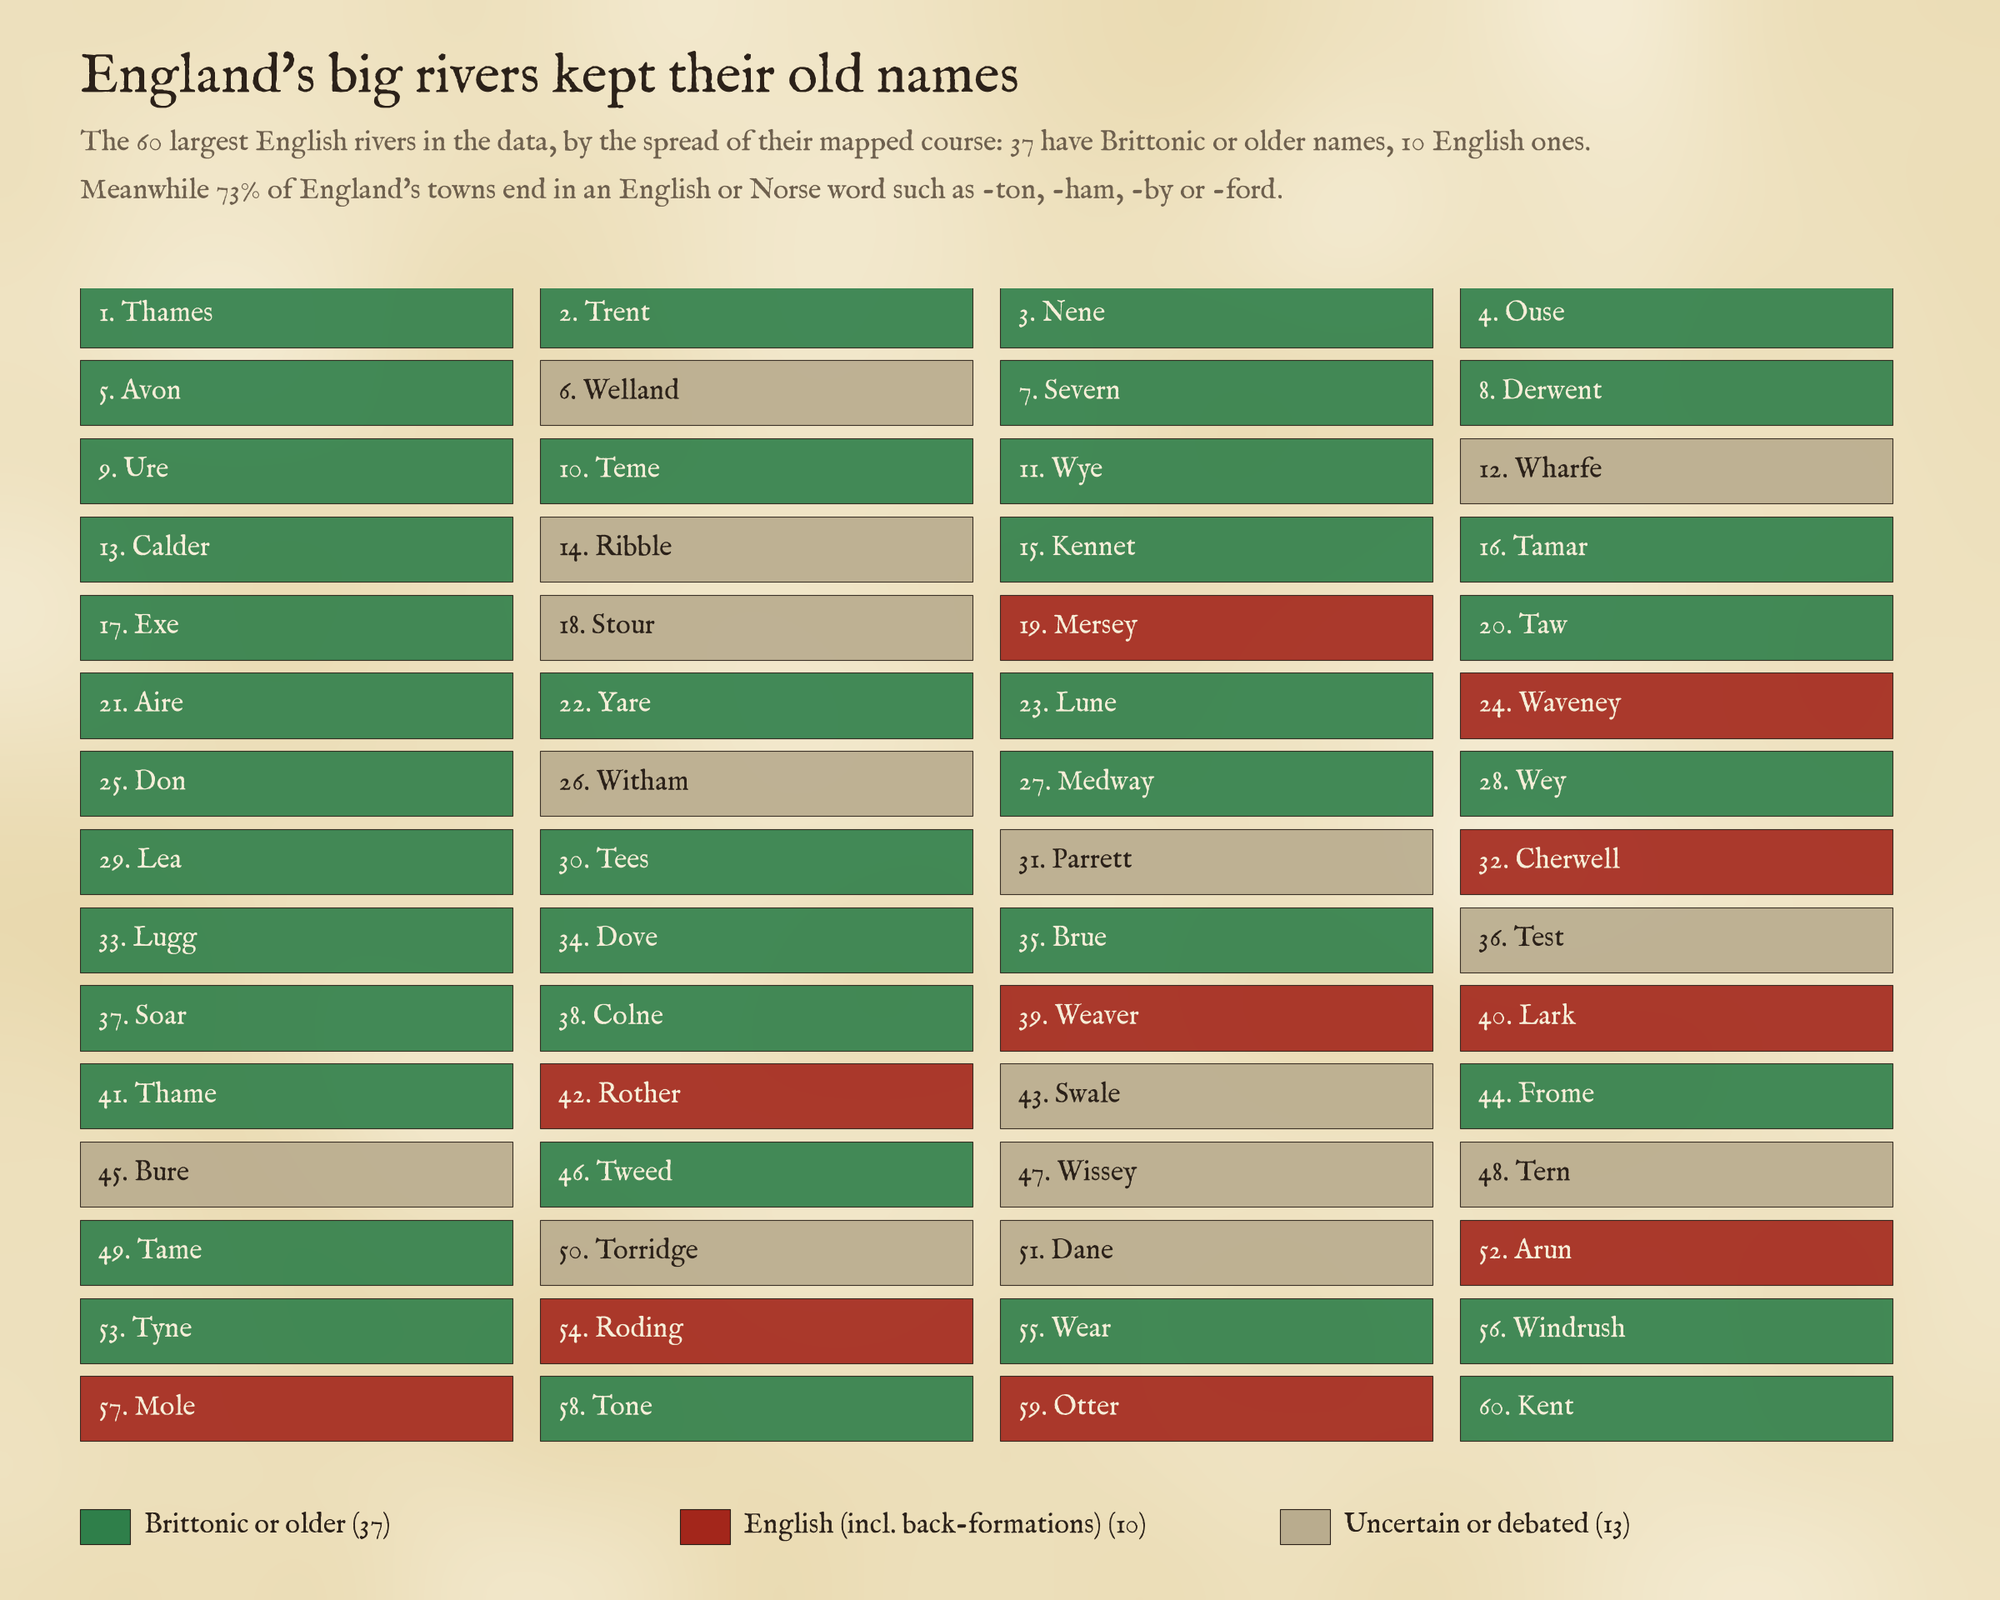
\includegraphics[width=\textwidth]{f_major.png}
\caption{The 60 largest English rivers in the data and the origin of their names.}\label{fig:major}\end{figure}

\begin{small}\begin{longtable}{rlrlp{6.6cm}}\caption{The 60 largest English rivers in the data, by the spread of their mapped course (km, a proxy for size), and the origin of the name after Ekwall (1928) and Watts (2004).}\label{tab:major}\\\toprule Rank & River & Spread & Origin & Note\\\midrule\endhead
1 & Thames & 184 & Brittonic or older & \\
2 & Trent & 107 & Brittonic or older & \\
3 & Nene & 106 & Brittonic or older & \\
4 & Ouse & 100 & Brittonic or older & \\
5 & Avon & 95 & Brittonic or older & \\
6 & Welland & 86 & uncertain & \\
7 & Severn & 77 & Brittonic or older & \\
8 & Derwent & 75 & Brittonic or older & \\
9 & Ure & 75 & Brittonic or older & \\
10 & Teme & 73 & Brittonic or older & \\
11 & Wye & 72 & Brittonic or older & \\
12 & Wharfe & 68 & uncertain & \\
13 & Calder & 67 & Brittonic or older & \\
14 & Ribble & 65 & uncertain & \\
15 & Kennet & 64 & Brittonic or older & \\
16 & Tamar & 58 & Brittonic or older & \\
17 & Exe & 58 & Brittonic or older & \\
18 & Stour & 56 & uncertain & \\
19 & Mersey & 55 & English & Old English, the boundary river\\
20 & Taw & 53 & Brittonic or older & \\
21 & Aire & 52 & Brittonic or older & \\
22 & Yare & 52 & Brittonic or older & \\
23 & Lune & 51 & Brittonic or older & \\
24 & Waveney & 51 & English & Old English, river by a quaking fen\\
25 & Don & 50 & Brittonic or older & \\
26 & Witham & 49 & uncertain & \\
27 & Medway & 49 & Brittonic or older & \\
28 & Wey & 49 & Brittonic or older & \\
29 & Lea & 48 & Brittonic or older & \\
30 & Tees & 47 & Brittonic or older & \\
31 & Parrett & 46 & uncertain & \\
32 & Cherwell & 46 & English & Old English wella, stream; first element uncertain\\
33 & Lugg & 45 & Brittonic or older & \\
34 & Dove & 45 & Brittonic or older & \\
35 & Brue & 41 & Brittonic or older & \\
36 & Test & 41 & uncertain & \\
37 & Soar & 41 & Brittonic or older & \\
38 & Colne & 39 & Brittonic or older & \\
39 & Weaver & 39 & English & Old English, winding river\\
40 & Lark & 38 & English & back-formation from Lackford\\
41 & Thame & 38 & Brittonic or older & \\
42 & Rother & 37 & English & back-formation from Rotherfield (the eastern Rother; the western Rother is from Rotherbridge)\\
43 & Swale & 37 & uncertain & \\
44 & Frome & 37 & Brittonic or older & \\
45 & Bure & 37 & uncertain & \\
46 & Tweed & 37 & Brittonic or older & \\
47 & Wissey & 36 & uncertain & \\
48 & Tern & 35 & uncertain & \\
49 & Tame & 35 & Brittonic or older & \\
50 & Torridge & 35 & uncertain & \\
51 & Dane & 34 & uncertain & \\
52 & Arun & 34 & English & back-formation from Arundel\\
53 & Tyne & 34 & Brittonic or older & \\
54 & Roding & 33 & English & from the Roding villages, Old English folk name\\
55 & Wear & 33 & Brittonic or older & \\
56 & Windrush & 33 & Brittonic or older & \\
57 & Mole & 33 & English & back-formation from Molesey\\
58 & Tone & 33 & Brittonic or older & \\
59 & Otter & 32 & English & Old English otor, otter\\
60 & Kent & 32 & Brittonic or older & \\
\bottomrule\end{longtable}\end{small}

\subsection{The roots}
Table~\ref{tab:roots} lists the root groups and the number of distinct rivers and streams in each. There are 10 Avons (6 in England, 4 in Scotland, where some may be Gaelic rather than Brittonic), 10 Esks, 6 Derwents, Darwens and Darents, and 15 Calders. In all 116 rivers and streams fall in the sixteen groups (Figures~\ref{fig:roots} and \ref{fig:avons}).

\begin{table}[tbp]\centering\small\caption{Root groups, the meaning given in the literature, the reading, and the number of distinct rivers and streams in the UK data.}\label{tab:roots}\begin{tabular}{p{4.2cm}p{6.6cm}lr}\toprule Names & Root and meaning & Reading & Rivers\\\midrule
Avon & Brittonic *abona, 'river' (Welsh afon) & certain & 10\\
Esk, Exe, Axe, Usk & Brittonic *isca, usually read as 'water' & probable & 16\\
Ouse & a Brittonic or older word for 'water' & probable & 5\\
Derwent, Darwen, Darent, Dart & Brittonic *derwā, 'oak': 'river where oaks grow' & certain & 11\\
Dee & Brittonic *dēwā, 'goddess, holy one' & probable & 4\\
Don & perhaps the goddess Dānu, or a word for water & probable & 5\\
Thames, Tame, Thame, Teme, Tamar, Team & a pre-English root *tam-, often read as 'dark' & probable & 8\\
Calder & Brittonic *caleto-dubron, 'hard (rocky) water' & certain & 15\\
Leven & Brittonic *lēβn-, 'smooth' & probable & 5\\
Aln, Alne, Allen, Ellen, Alun & a pre-English root *alaun-, meaning uncertain & probable & 15\\
Frome & Brittonic *frām, 'fair, fine, brisk' & probable & 6\\
Kennet, Kent & a pre-English root of uncertain meaning (Roman Cunetio) & probable & 2\\
Colne, Clun & pre-English, meaning unknown & probable & 5\\
Wye, Wey & pre-English, meaning unknown & probable & 5\\
Trent & Brittonic, often read as 'the trespasser', the river that floods & probable & 1\\
Severn & pre-English (Latin Sabrina, Welsh Hafren), meaning unknown & certain & 3\\
\bottomrule\end{tabular}\end{table}

\begin{figure}[tbp]\centering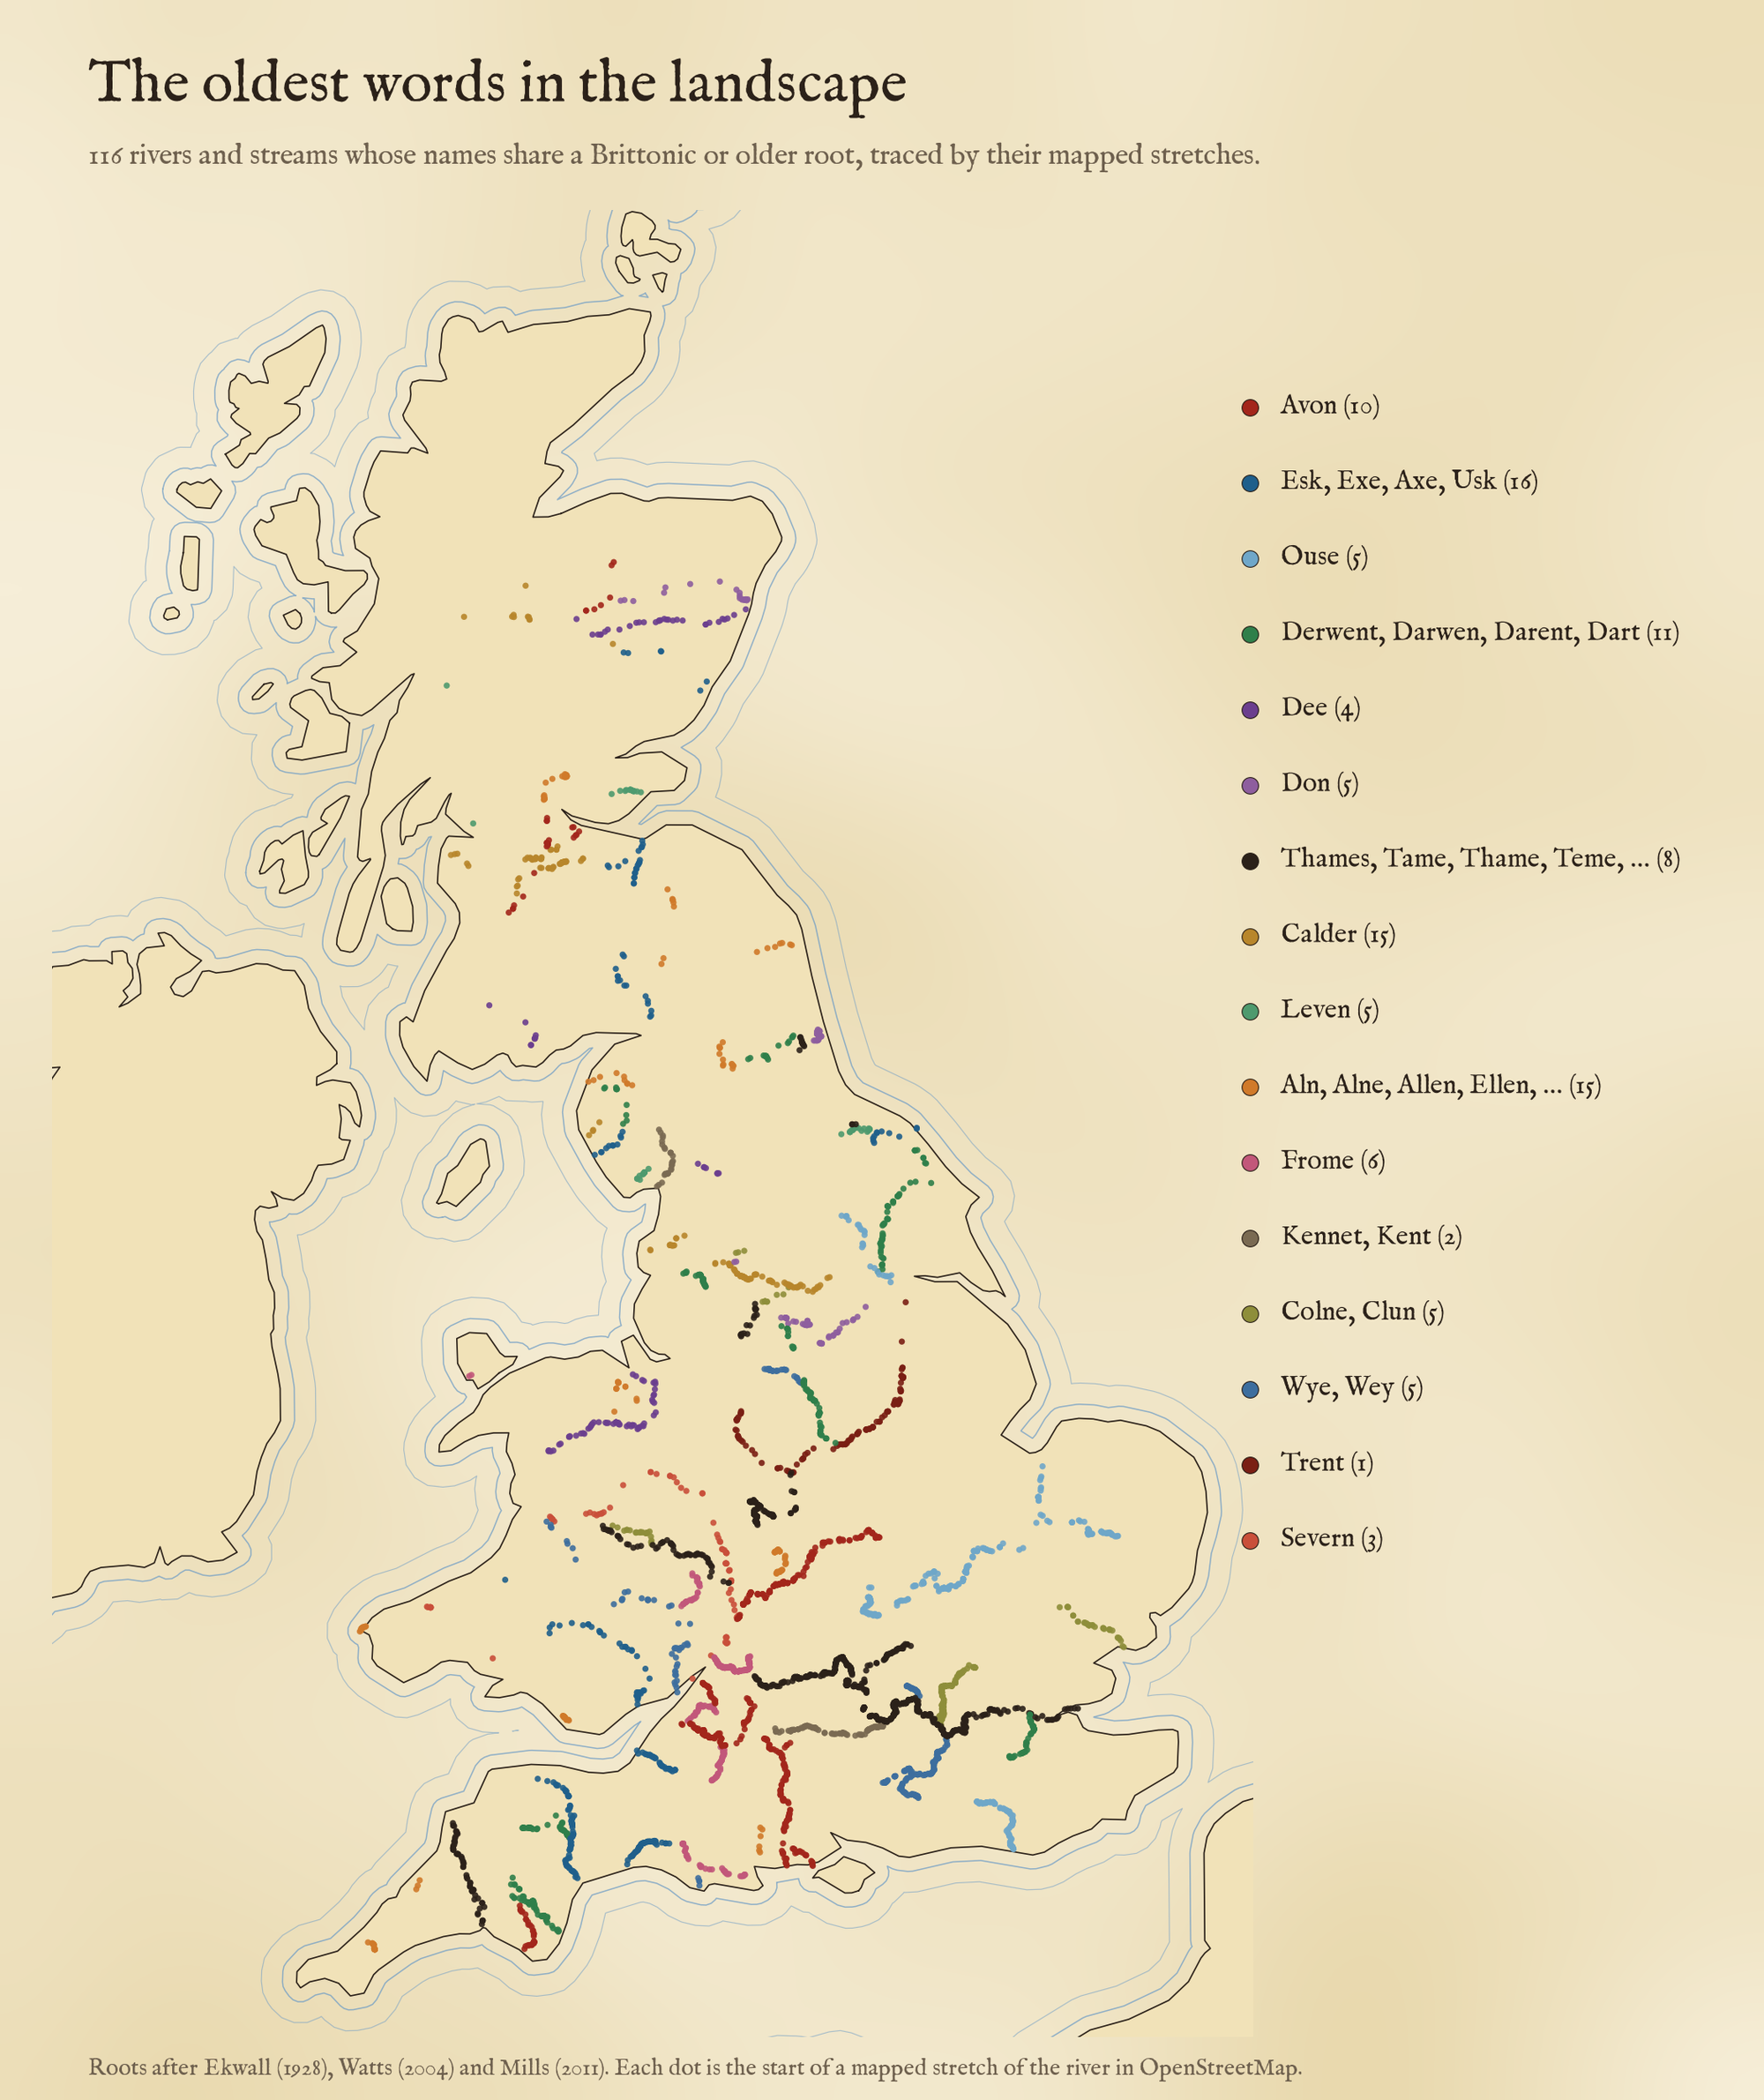
\includegraphics[width=0.85\textwidth]{f_roots.png}
\caption{The courses of the rivers in the sixteen root groups.}\label{fig:roots}\end{figure}

\begin{figure}[tbp]\centering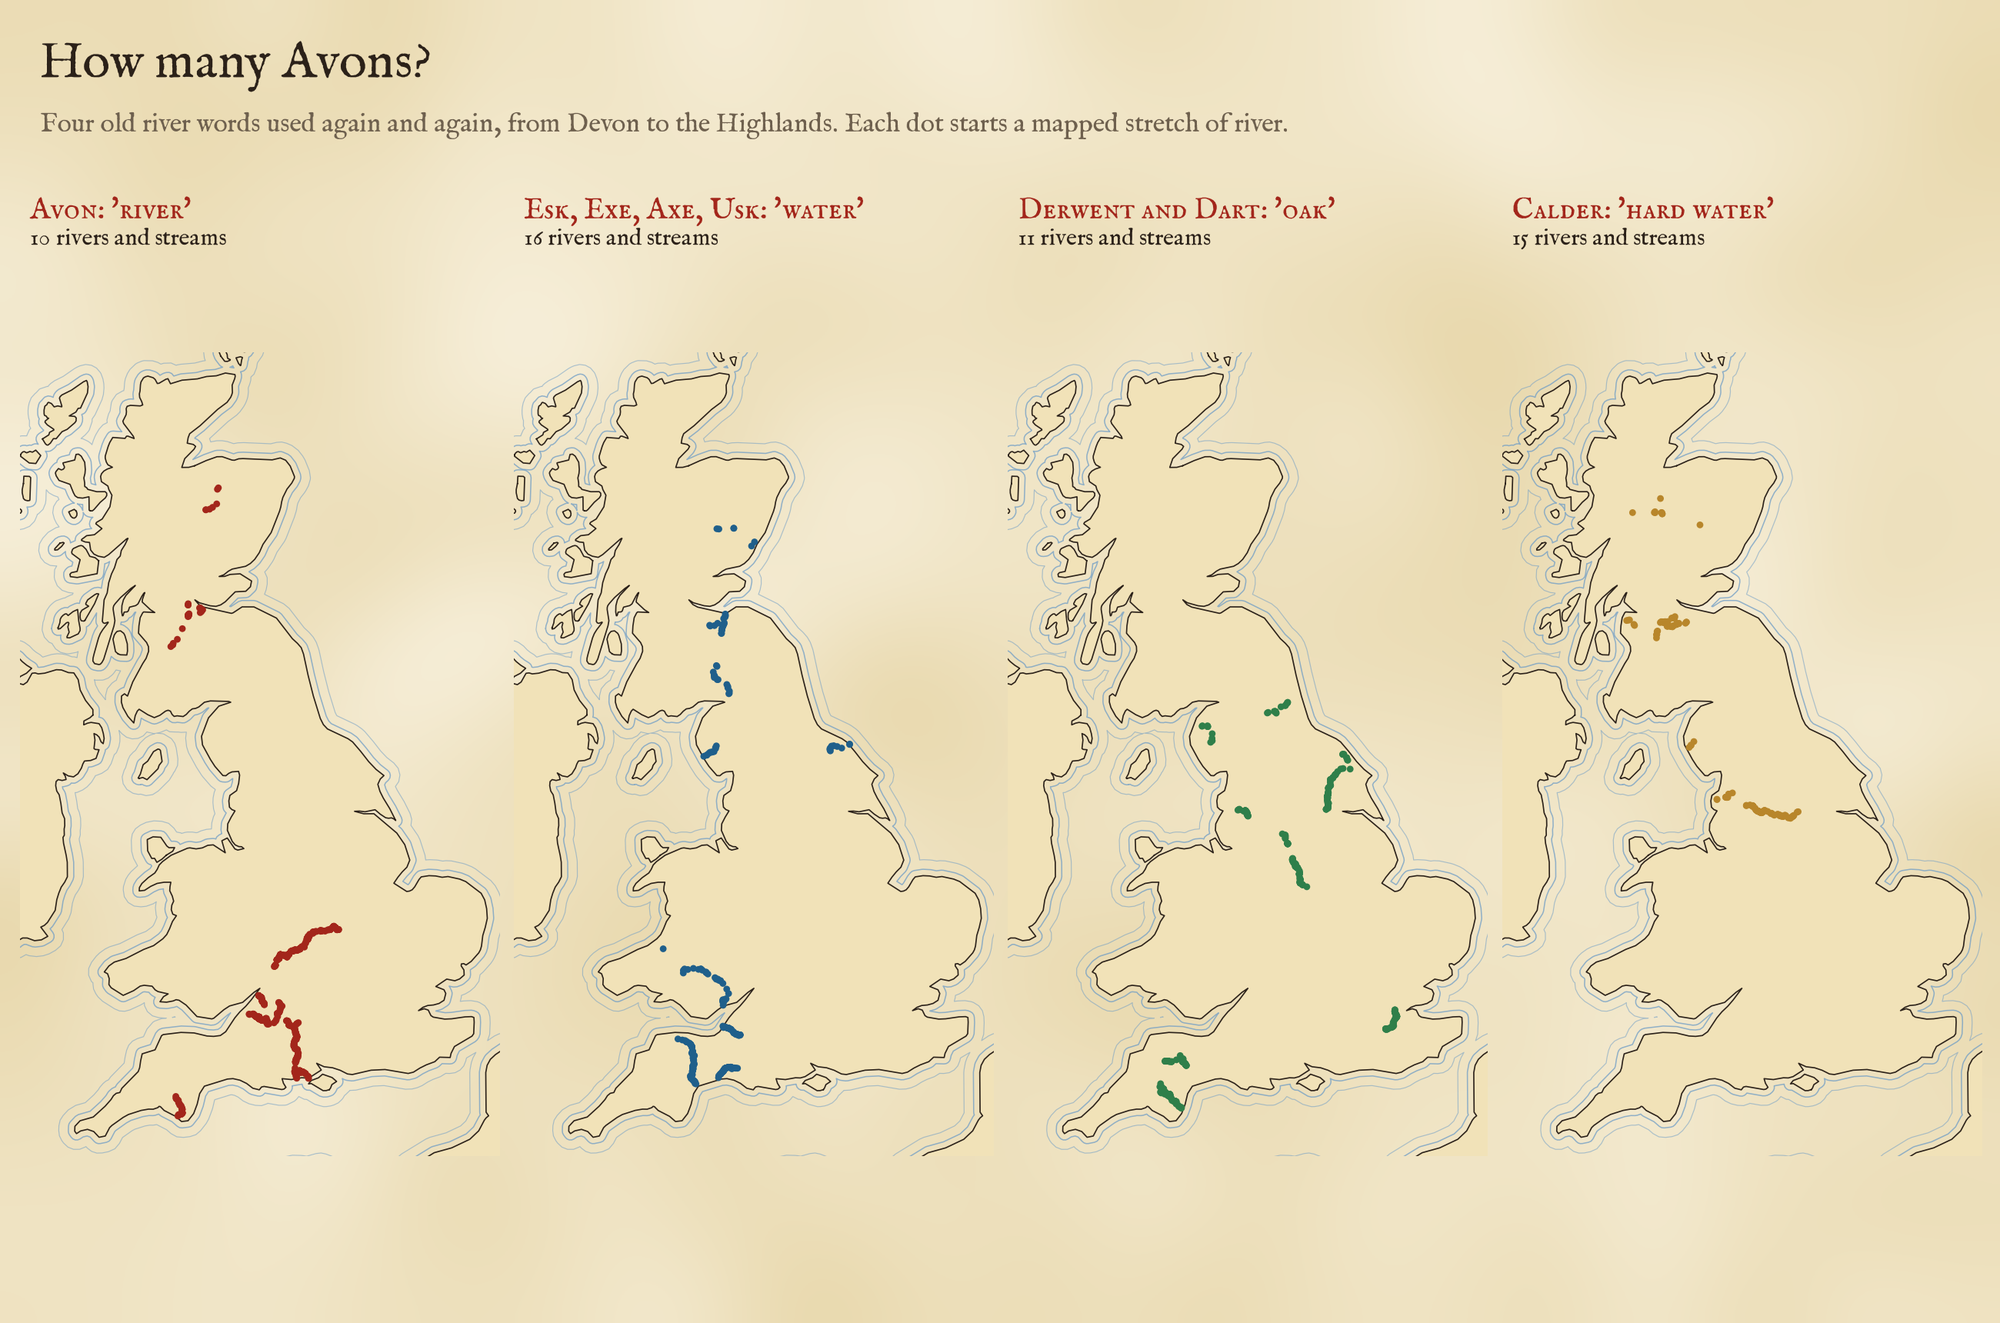
\includegraphics[width=\textwidth]{f_avons.png}
\caption{Avon; Esk, Exe, Axe and Usk; Derwent and Dart; and Calder.}\label{fig:avons}\end{figure}

\subsection{The generic words}
Burn (5,792), allt (4,263), brook (3,284), beck (2,969), gill (1,760), nant (1,480), sike (1,136), water (825) and afon (793) are the commonest generics (Figure~\ref{fig:generics}). In Wales \citep{owen2007} 86.3\% of streams named with \textit{nant}, \textit{afon}, \textit{brook} or \textit{river} are \textit{nant} or \textit{afon}. In Scotland \citep{watson1926} Gaelic \textit{allt} and \textit{abhainn} account for 47.9\% of the four main generics overall, 86.2\% in Highland, 98.8\% in the Western Isles, 16.7\% in Aberdeenshire and none in the Scottish Borders or Dumfries and Galloway, where the streams are burns, waters and sikes (the Gaelic past of Galloway shows instead in names in \textit{Pol-}, from Gaelic \textit{poll}, such as Polmaddy Burn). Local words follow local landscapes: 26 rhynes in Somerset and 8 lodes in Cambridgeshire.

\begin{figure}[tbp]\centering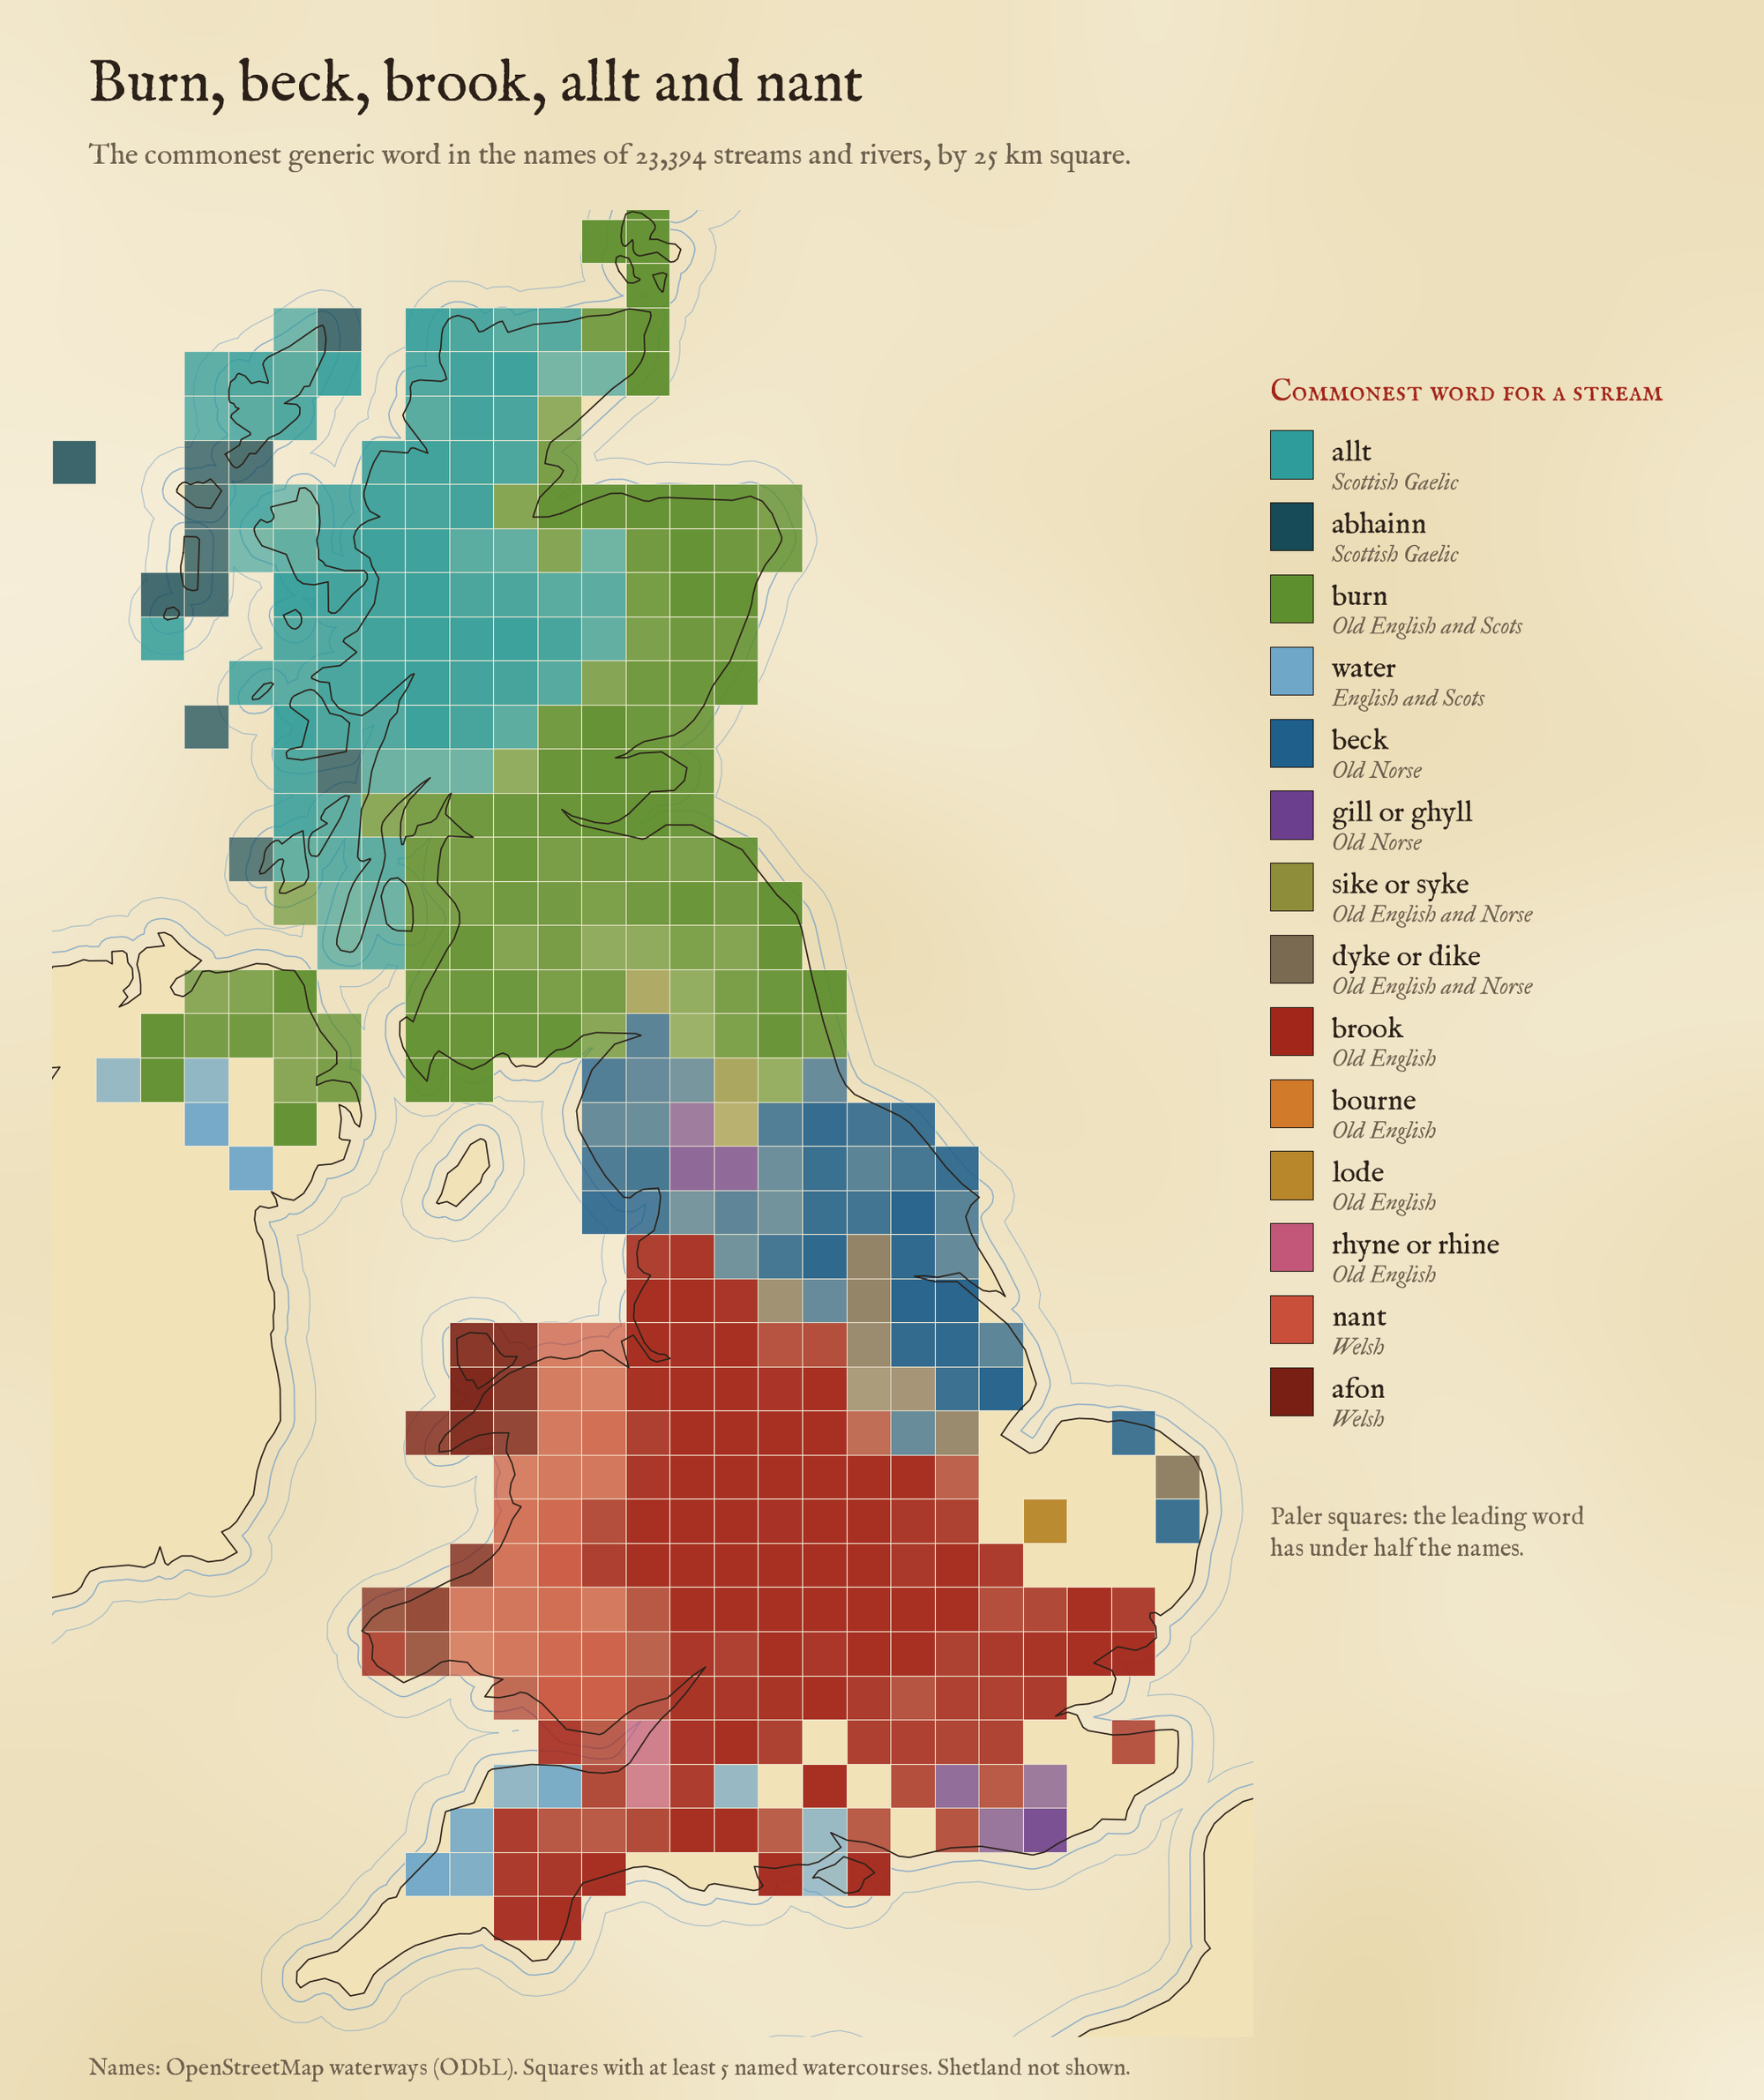
\includegraphics[width=0.85\textwidth]{f_generics.png}
\caption{The commonest generic word in each 25 km square (at least five named watercourses).}\label{fig:generics}\end{figure}

\subsection{The beck line}
Becks outnumber brooks in England north of about 53.75\textdegree{}N (Figure~\ref{fig:beck}). The 5th percentile of beck latitudes is 53.56\textdegree{}N and the 95th percentile of brook latitudes 53.74\textdegree{}N, so the change is sharp. It is not only latitude: in Lincolnshire and Nottinghamshire (median place latitude 53.19\textdegree{}N) there are 115 becks to 26 brooks (81.6\% becks), against 0 becks to 755 brooks in Cheshire, Staffordshire, Shropshire and Greater Manchester (52.90\textdegree{}N). Lincolnshire (96.0\%) and Norfolk (94.7\%) are almost all beck. Derbyshire and Leicestershire, within the Danelaw of the Five Boroughs, have 2 becks to 300 brooks, so the beck tracks dense Norse-speaking settlement rather than the political boundary.

\begin{figure}[tbp]\centering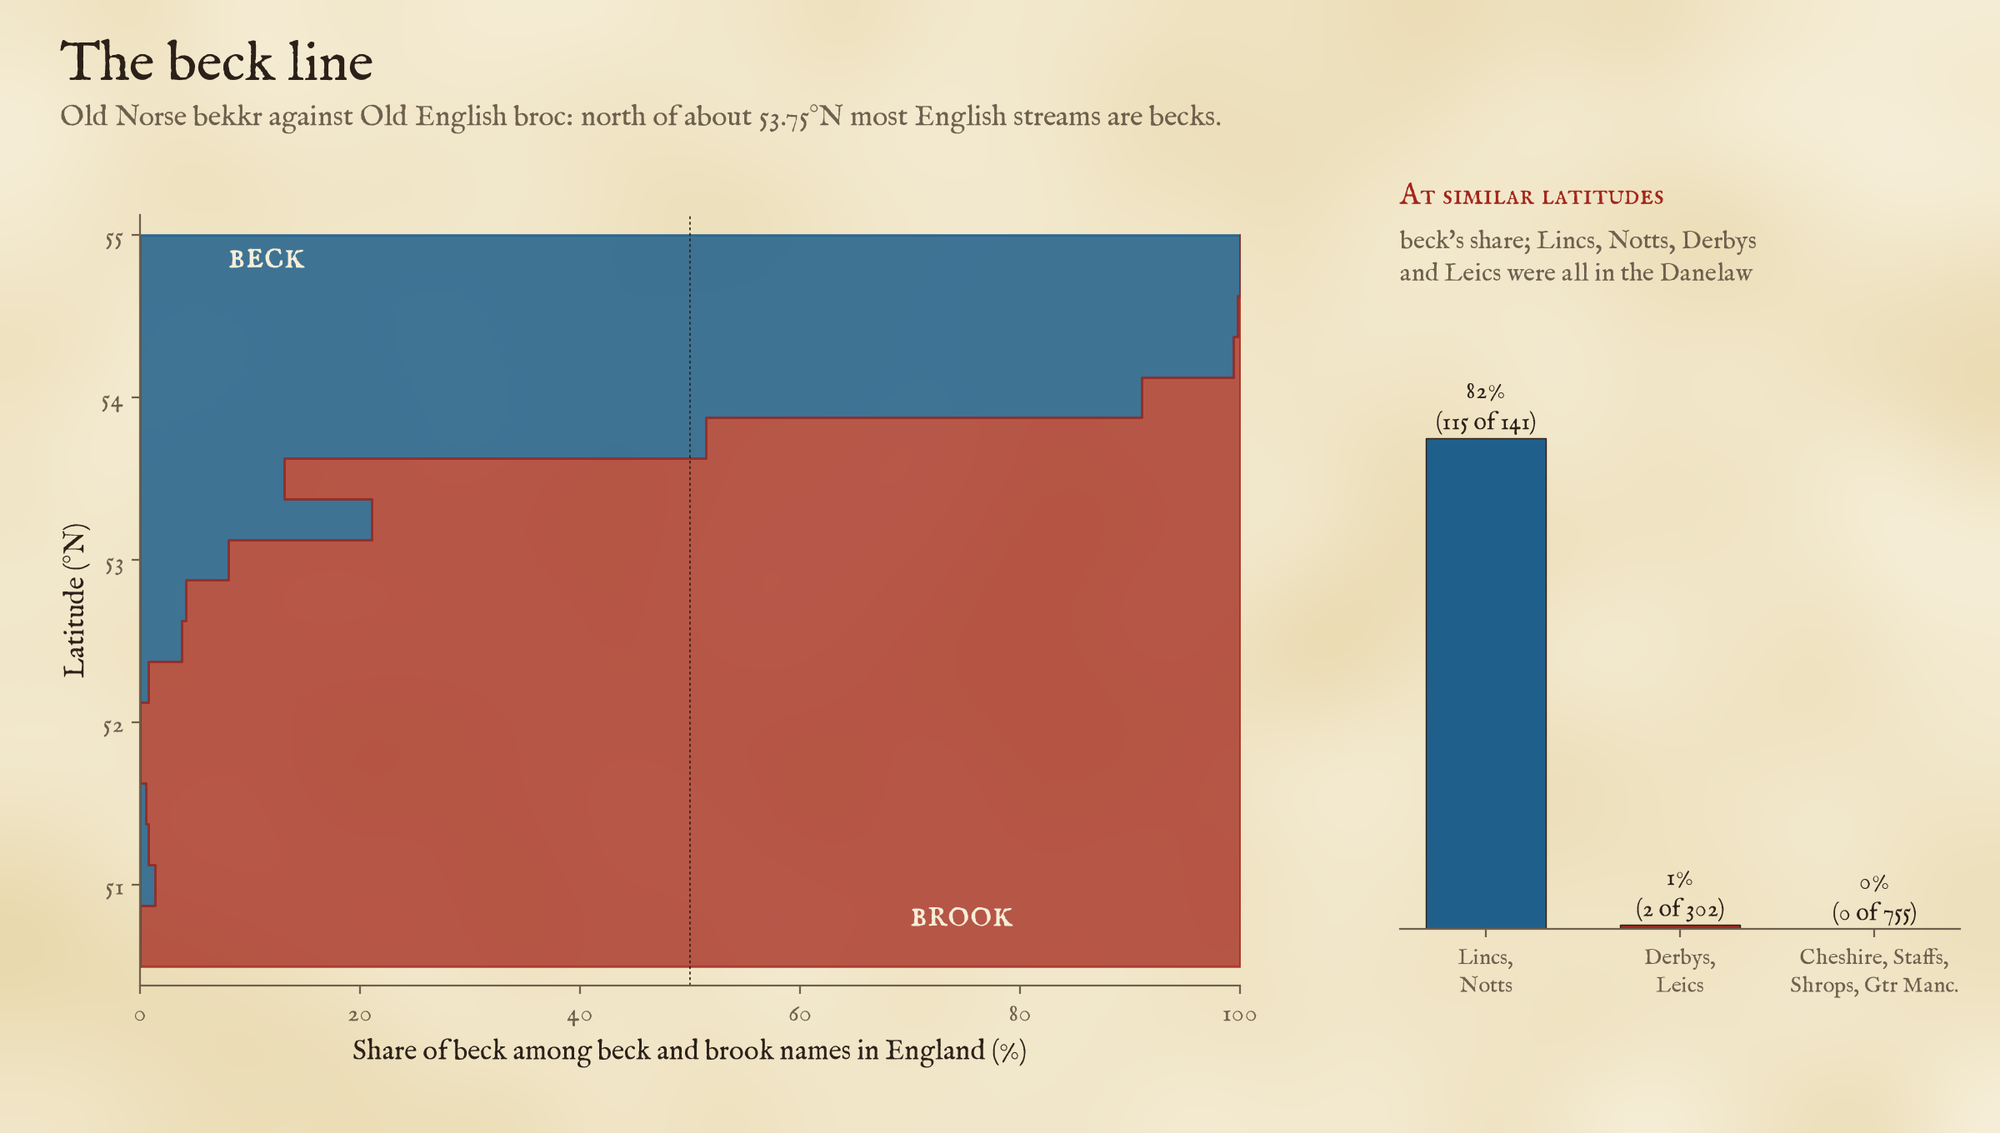
\includegraphics[width=\textwidth]{f_beck.png}
\caption{Beck against brook by latitude in England (left) and in eastern and western counties at similar latitudes (right).}\label{fig:beck}\end{figure}

\section{Limitations}
The etymologies are the standard ones, applied without re-examining early spellings; several are debated (the meaning of the \textit{Tam-} root and of \textit{*isca}, the Scottish Avons, Stour, Wharfe, the first element of Cherwell) and the origin classes of the 60 largest rivers should be read as a summary of the literature, not a new judgement. OpenStreetMap's naming of small streams is uneven between regions and mappers, and many small streams are unnamed in it; the generic shares describe named streams in the map, not the whole historical record. The size ranking is a proxy: rivers mapped in a few long ways score low, so some long rivers, such as the Eden in Cumbria, fall outside the 60, and the River Tweed counts only for its English stretch. A ranking by true length would change the list at the margin. The town test reads only word endings. The joining of ways into rivers was checked by hand only for the root groups.

\section{Conclusion}
Mapped from an open gazetteer, Britain's river names show both layers that the place-name literature describes: a scatter of very old names, Avon, Esk, Derwent, Calder, Dee, under an English landscape of towns, and an everyday vocabulary of streams that still follows the old language boundaries, Gaelic in the Highlands, Welsh in Wales, and the Norse beck where Scandinavian settlers were thickest.

\section*{Data and code availability}
The interactive map is at \url{https://maps.tristanhotham.com/river-names/}. Code, the root rules, the hand assignments and the derived tables are at \url{https://github.com/Tristan-Hotham/river-names} and archived with this paper at https://doi.org/10.5281/zenodo.24063209. The river tables are derived from OpenStreetMap (\copyright{} OpenStreetMap contributors) and released under the Open Database Licence; text and figures CC BY 4.0; code MIT. County boundaries from the ONS (Open Government Licence v3.0).

\section*{AI statement}
I wrote the text, with drafting and editing assistance from Claude (Anthropic), which also helped prepare the analysis code. I reviewed and checked all text and results.

\begin{thebibliography}{10}
\bibitem[Bast and Buchhold(2017)]{bast2017} Bast, H. and Buchhold, B. (2017) QLever: a query engine for efficient SPARQL+Text search. \textit{Proceedings of the 2017 ACM Conference on Information and Knowledge Management (CIKM)}, 647 to 656.
\bibitem[Ekwall(1928)]{ekwall1928} Ekwall, E. (1928) \textit{English River-Names}. Oxford: Clarendon Press.
\bibitem[Gelling and Cole(2000)]{gelling2000} Gelling, M. and Cole, A. (2000) \textit{The Landscape of Place-Names}. Stamford: Shaun Tyas.
\bibitem[Mills(2011)]{mills2011} Mills, A. D. (2011) \textit{A Dictionary of British Place-Names}, revised edn. Oxford: Oxford University Press.
\bibitem[Owen and Morgan(2007)]{owen2007} Owen, H. W. and Morgan, R. (2007) \textit{Dictionary of the Place-Names of Wales}. Llandysul: Gomer.
\bibitem[Watson(1926)]{watson1926} Watson, W. J. (1926) \textit{The History of the Celtic Place-Names of Scotland}. Edinburgh: Blackwood.
\bibitem[Watts(2004)]{watts2004} Watts, V. (ed.) (2004) \textit{The Cambridge Dictionary of English Place-Names}. Cambridge: Cambridge University Press.
\end{thebibliography}
\end{document}
